% !TEX encoding = UTF-8 Unicode
% !TEX TS-program = pdflatex
% !TEX TS-program = xelatex

\DeclareOldFontCommand{\rm}{\normalfont\rmfamily}{\mathrm}
\DeclareOldFontCommand{\sf}{\normalfont\sffamily}{\mathsf}
\DeclareOldFontCommand{\tt}{\normalfont\ttfamily}{\mathtt}
\DeclareOldFontCommand{\bf}{\normalfont\bfseries}{\mathbf}
\DeclareOldFontCommand{\it}{\normalfont\itshape}{\mathit}
\DeclareOldFontCommand{\sl}{\normalfont\slshape}{\@nomath\sl}
\DeclareOldFontCommand{\sc}{\normalfont\scshape}{\@nomath\sc}
\DeclareRobustCommand*\cal{\@fontswitch\relax\mathcal}
\DeclareRobustCommand*\mit{\@fontswitch\relax\mathnormal}

\documentclass[%
	12pt, 
	a4paper,
	oneside, 
	ngerman,
	bibtotoc,
	dvipsnames,
	table,
]{scrartcl}

\usepackage{wrapfig} 
\usepackage[printonlyused]{acronym}

%\usepackage{tikz}
\usepackage{amssymb,amsmath}
\usepackage{ifxetex,ifluatex}
\usepackage{fixltx2e} % provides \textsubscript
%\usepackage{struktex}

\ifxetex
  \usepackage{fontspec,xltxtra,xunicode}
  \defaultfontfeatures{Mapping=tex-text,Scale=MatchLowercase}
  \newcommand{\euro}{€}
    \usepackage{polyglossia} % -ak-
  \setmainlanguage[%
  	spelling=new,%old
  	latesthyphen=true,%false
	%babelshorthands=true,%false
	]{german} % -ak-
  %\setmainlanguage[variant=american]{english} % -ak-
  \usepackage{xecolor}
\else
  \ifluatex
    \usepackage{fontspec}
    \defaultfontfeatures{Mapping=tex-text,Scale=MatchLowercase}
    \newcommand{\euro}{€}
    \usepackage[ngerman]{babel} % -ak-
    \usepackage{color}
  \else
    \usepackage[utf8]{inputenc}
    \usepackage[TS1,T1]{fontenc} % -ak- T1 für \textdblquotedown
    \usepackage{lmodern} % -ak-
%   \usepackage{tgbonum}	% Bookman
%   \usepackage{tgpagella}	% Palatino
%   \usepackage{tgtermes}	% Times
%   \usepackage{tgschola}	% Century Schoolbook
%   \usepackage{iwona}	% 
%   \usepackage{anttor}
    \usepackage[ngerman]{babel}
    \usepackage{color}    
  \fi
\fi


% Format A4
\typearea[3mm]{13}

% Format A5
%\setlength{\paperwidth}{14.8cm}
%\setlength{\paperheight}{21cm}
%\typearea[2mm]{13}

% Format Taschenbuch
%\setlength{\paperwidth}{12cm}
%\setlength{\paperheight}{19cm}
%\typearea[2mm]{12}

% Format iPad
%\setlength{\paperwidth}{14,5cm}
%\setlength{\paperheight}{19cm}
%\typearea{13}

% Format iPod
%\setlength{\paperwidth}{9cm}
%\setlength{\paperheight}{11,5cm}
%\typearea{14}



\ifxetex
\else
	\usepackage{microtype}
\fi
\raggedbottom
\emergencystretch 0.8em

\definecolor{gcolor}{rgb}{0,0,0} % schwarz

%\usepackage{natbib}
%\bibliographystyle{plainnat}

%\usepackage{biblatex}

%\bibliography{$biblio-files$}

%\usepackage{fancyvrb}

% Redefine labelwidth for lists; otherwise, the enumerate package will cause
% markers to extend beyond the left margin.
\makeatletter\AtBeginDocument{%
  \renewcommand{\@listi}
    {\setlength{\labelwidth}{4em}}
}\makeatother
\usepackage{enumerate}

\usepackage{ctable}
\usepackage{float} % provides the H option for float placement

\usepackage{url}

\usepackage{graphicx}



% We will generate all images so they have a width \maxwidth. This means
% that they will get their normal width if they fit onto the page, but
% are scaled down if they would overflow the margins.
%\makeatletter
%\def\maxwidth{\ifdim\Gin@nat@width>\linewidth\linewidth
%\else\Gin@nat@width\fi}
%\makeatother
%\let\Oldincludegraphics\includegraphics
%\renewcommand{\includegraphics}[1]{\Oldincludegraphics[width=\maxwidth]{#1}}

\usepackage{verbatim}

\usepackage{nameref}


\newcommand{\seclabel}[1]{
\label{sec:#1}
}

\newcommand{\secnameref}[1]{
\nameref{sec:#1}
}

\newcommand{\secnamerefn}[1]{
\ref{sec:#1}: \nameref{sec:#1}
}

\newcommand{\secnamerefnpb}[1]{
Kapitel\secnamerefn{#1}auf Seite \pageref{sec:#1}
}

\newcommand{\secnamerefnpbf}[1]{
Kapitel\secnamerefn{#1}auf Seite \pageref{sec:#1}.
}

\newcommand{\secnamerefnp}[1]{
(Kapitel\secnamerefn{#1}auf Seite \pageref{sec:#1})
}


\newenvironment{myindentpar}[1]%
{\begin{list}{}%
	{\setlength{\leftmargin}{#1}}%
	   	\item[]%
   	}
{\end{list}}

\usepackage{caption}
\DeclareCaptionType{mycapequ}[][List of equations]
\captionsetup[mycapequ]{labelformat=empty}

\usepackage{float}
%\floatstyle{boxed}
\restylefloat{figure}

\newcommand{\figref}[1]{
Abb.~\ref{fig:#1}
}

\newcommand{\figreflong}[1]{
Abbildung~\ref{fig:#1}
}

\newcommand{\figrefp}[1]{
\figref{#1} auf Seite~\pageref{fig:#1}
}


% @acuda
% change to alternative figure numbering
% default:  in book class figures are numbered per chapter
%           in article class figures are numbred continuously
%
% change book-class default to continuosly behavior:
% \usepackage{chngcntr}
% \counterwithout{figure}{chapter}
%
% change article-class default to per chapter (section) style:
\usepackage{chngcntr}
%\counterwithin{figure}{section}


% @acuda
% generate new appendix behavior
% now add caption to toc without numbering
\let\Oldappendix\appendix
\def\appendix{
	\Oldappendix
	%\phantomsection 
	\addcontentsline{toc}{section}{Anhang}
	\renewcommand\refname{Anhang} \section*{Anhang}
}

% @acuda #####################
%add for centered captions following options: justification=justified, singlelinecheck=false
\usepackage[font=small, labelfont=bf]{caption}
\usepackage{subcaption}

\KOMAoptions{parskip=half}
%\addtokomafont{caption}{\footnotesize} %lable captions smaller...


\usepackage{blindtext} 

\usepackage{bibgerm}
%\usepackage{titlesec}	%clearpage (newpage with correct floating enviroment) before sections
\newcommand{\sectionbreak}{\clearpage}



\ifxetex
  \usepackage[setpagesize=false, % page size defined by xetex
              unicode=false, % unicode breaks when used with xetex
              xetex,
              bookmarks=true,
              pdfauthor={$author-meta$},
              pdftitle={$title-meta$},
              colorlinks=true,
              urlcolor=blue,
              linkcolor=blue]{hyperref}
\else
  \usepackage[unicode=true,
              bookmarks=true,
              pdfauthor={$author-meta$},
              pdftitle={$title-meta$},
              colorlinks=false,
              urlcolor=blue,
              linkcolor=blue]{hyperref}
\fi
\hypersetup{breaklinks=true, pdfborder={0 0 0}}

\setlength{\emergencystretch}{3em}  % prevent overfull lines


\usepackage{textcomp}

\usepackage{csquotes}

\usepackage{multirow}
\usepackage{pdflscape}

\setcounter{tocdepth}{3}


%%%% Eigene Kopf und Fußzeile %%%%%%%%%%%%%%%% 
%\usepackage{scrpage2}%                              Package laden 
%\pagestyle{scrheadings}%                           SCRPAGE2 Style aktivieren 
%\clearscrheadfoot%                                    lösche alle Kopf und Fußzeilen 
%\setheadwidth{textwithmarginpar}%             für textbreite+rand 
%\automark{chapter}%                                    Autoerkenneung Chapter 
%\ohead{\textbf{\pagemark}}%                      Seitenzahl 
%\renewcommand{\chaptermark}[1]{\markright{\ #1}} %löscht die Nummerierung von Chapter 
%\ihead{\textbf{\rightmark}} 
%%%%%%%%%% Striche Kopfzeile %%%%%%%%%%%%% 
%\setheadtopline{2pt}[\color{blue}] 
%\setheadsepline{1pt}[\color{blue}] 



%\usepackage[
%	automark,
%	headsepline,                %% Separation line below the header
%	%footsepline,               %% Separation line above the footer
%	markuppercase
%]{scrlayer-scrpage}
%\automark[%
%	%subsection  % durch renewcommand gelöst?
%]{section}
%\pagestyle{scrheadings}
%\renewcommand{\sectionmark}[1]{\markright{\ #1}} %löscht die Nummerierung von Chapter 

%\lefoot{}                      %% Bottom left on even pages
%\lofoot{}                      %% Bottom left on odd pages
%\refoot{}                      %% Bottom right on even pages
%\rofoot{}                      %% Bottom right on odd pages
%\cfoot{--~\pagemark~--}        %% Bottom center
 
%\lehead{\bfseries\pagemark}    %% Top left on even pages
%\lohead{\bfseries\headmark}    %% Top left on odd pages
%\rehead{\bfseries\headmark}    %% Top right on even pages
%\rohead{\headmark}    %% Top right on odd pages
%\chead{}                       %% Top center
%\renewcommand{\subsectionmark}[1]{\markright{\ #1}} %löscht die Nummerierung von Chapter 


%%%%%%%%%%%%%%%%%%%%%%%%%%%%%%%%%%%%%%%%%%%%%%%%%%%%%
% C M D :   E I G E N N A M E N
%%%%%%%%%%%%%%%%%%%%%%%%%%%%%%%%%%%%%%%%%%%%%%%%%%%%%

\newcommand{\en}[1]{%
\glqq\textit{#1}\grqq%
}


\usepackage{listings}
%\input{listings-python-setup}
%\input{python-function-definition-setup}

\usepackage{setspace}	%zeilenabstand

\makeatletter
\newcommand{\MSonehalfspacing}{%
  \setstretch{1.44}%  default
  \ifcase \@ptsize \relax % 10pt
    \setstretch {1.448}%
  \or % 11pt
    \setstretch {1.399}%
  \or % 12pt
    \setstretch {1.433}%
  \fi
}

\newcommand{\MSdoublespacing}{%
  \setstretch {1.92}%  default
  \ifcase \@ptsize \relax % 10pt
    \setstretch {1.936}%
  \or % 11pt
    \setstretch {1.866}%
  \or % 12pt
    \setstretch {1.902}%
  \fi
}
\makeatother


\onehalfspacing



%%%%%%%%%%%%%%%%%%%%%%%%%
% TEXT ANNOTATIONS		
%%%%%%%%%%%%%%%%%%%%%%%%%

\newcommand{\note}[1]{
\textcolor{orange}{\textbf{Notiz:} #1}
}

\makeatletter
\newcommand{\todo}[1]{
\textcolor{blue}{\textbf{ToDo:} #1}
}




\let\oldcite\cite%
\renewcommand{\cite}[2][]{%
	\ifx&#1&%
		\mbox{\oldcite{#2}}%
	\else%
		\mbox{\oldcite[#1]{#2}}%
	\fi%
}

\newcommand*{\eqcite}[2][]{%
	\vadjust{%
	    \smallskip
	    \hbox to \linewidth{\hfill%
			\ifx&#1&%
				\cite{#2}%
			\else%
				\cite[#1]{#2}%
			\fi%
	    }%
	}%
}%

% Mit diesem Paket können Farben innerhalb von Tabellen verwendet werden. 
% Es können Spalten, Zeile oder einzelne Zellen eingefärbt werden.
\usepackage{colortbl}

\DeclareUnicodeCharacter{20AC}{\euro}

\definecolor{mygreen}{RGB}{28,172,0} % color values Red, Green, Blue
\definecolor{mylilas}{RGB}{170,55,241}

\lstset{language=Matlab,%
	%basicstyle=\color{red},
	breaklines=true,%
	morekeywords={matlab2tikz},
	keywordstyle=\color{blue},%
	morekeywords=[2]{1}, keywordstyle=[2]{\color{black}},
	identifierstyle=\color{black},%
	stringstyle=\color{mylilas},
	commentstyle=\color{mygreen},%
	showstringspaces=false,%without this there will be a symbol in the places where there is a space
	numbers=left,%
	numberstyle={\tiny \color{black}},% size of the numbers
	numbersep=9pt, % this defines how far the numbers are from the text
	emph=[1]{for,end,break},emphstyle=[1]\color{blue}, %some words to emphasise
	%emph=[2]{word1,word2}, emphstyle=[2]{style},    
}


\begin{document}

\thispagestyle{plain}
\begin{titlepage}
\typearea[3mm]{16}
\begin{center}
%\begin{figure}[H]
\centering

\includegraphics[scale=0.57]{grafic/logo_hhn_titlepage_new} \\
%
\includegraphics[scale=2.2]{grafic/logo_hhn_titlepage} \\
\vspace{0.2cm}
\large Fakultät für Mechanik und Elektronik
%\end{figure}
\vspace{0.5cm}
\hrule

\vspace{2.5cm}

\LARGE{\textbf{\scshape{Ausgewählte Kapitel der Robotik}}}\\
\vspace{2.1cm}

\Huge{\textbf{Abschlussprojekt\\zur Vorlesung}} \\
\vspace{2.1cm}

\Large{\textbf{\scshape{Gruppe 4}}}\\
\vfill

%\begin{figure}[H]
%\setlength{\extrarowheight}{2pt}%
\begin{table}[!h]
\newlength{\myl}
\settowidth{\myl}{Lecturer:  }
\hspace{-\myl}
\centering
\large
% \begin{tabular}{|p{3cm}|p{0.09\linewidth}p{0.15\linewidth}p{0.09\linewidth}|}
\begin{tabular}{p{2.5cm} p{5.3cm} p{1.8cm}} %{llr}
\textbf{Dozent:} & \multicolumn{2}{l}{Prof. Andreas Hoch} \\
\textbf{Betreuer:} & \multicolumn{2}{l}{B.Eng. Fabian Finkbeiner} \\
			     &              	  		&  			\\ 
\textbf{Autoren:}& Semyon Kondratev	& 207612	    \\
	             & Lisa-Franziska Schäfer	& 199318 	\\
\end{tabular}
\end{table}
%\end{figure}

\large
\vspace{0.5cm}
%\vfill
\hrule
%\vspace{0.5cm}
\normalsize
Abgabedatum: 21. Februar 2022%\today 

\end{center}


\thispagestyle{empty}
	
\end{titlepage}

%\input{urheberschaft}

\typearea[3mm]{15}
\pagenumbering{roman}


%%%%%%%%%%%%%%%%%%%%%%%%%%%%%%%%%%%%%%%%%%%%%%%%%%%%%
% T O C
%%%%%%%%%%%%%%%%%%%%%%%%%%%%%%%%%%%%%%%%%%%%%%%%%%%%%
\begingroup
\tableofcontents
\endgroup

\clearpage
\pagenumbering{arabic}
%\setcounter{page}{2} % reset page counter -> titlepage is not counted


\section{Einleitung}

Im Rahmen des Abschlussprojekts zur Vorlesung Ausgewählte Kapitel der Robotik sollen verschiedene Aufgaben rund um den Roboter UR10 der Firma Universal Robots bearbeitet werden.
Zunächst soll das Modell des Roboters in Matlab Simscape nachgebildet werden.
Dazu können die step-Dateien des Roboters verwendet werden, welche auf einigen Webseiten als kostenloser Download zur Verfügung stehen.
Die Massen und Trägheiten der Armteile bzw. Gelenke sollen dabei abgeschätzt werden.
Als Nächstes soll die zugewiesene Bewegungssequenz aus dem Beispielvideo dargestellt werden.
Die Bewegung umfasst dabei eine etwa drei Sekunden lange \en{Point to Point} Bewegung des UR10.
Eine weitere Aufgabe ist, die Drehmomentverläufe der Antriebe des Modells in Simscape auszugeben.
Als Letztes sollen die von der Simulation berechneten Drehmomente mittels einer Vergleichsrechnung mit Newton-Euler-Verfahren überprüft werden. 


Beim UR10 handelt es sich um einen 6-Achs Roboterarm, welcher in der Abbildung \ref{fig:ur10} zu sehen ist.
Sein Aufbau ist an einen menschlichen Arm angelehnt, wodurch er nahezu jede Position in seinem Arbeitsraum erreichen kann.
Er ist der größte der UR-Familie und kann Lasten von bis zu 10\,kg bei einem Arbeitsradius von bis zu 1300\,mm bewegen.
Dies ermöglicht ihm ein breites Anwendungsspektrum in der Maschinenbestückung, Palettierung und Verpackung.\cite{ur}

\begin{figure}[!htbp]
	\centering
	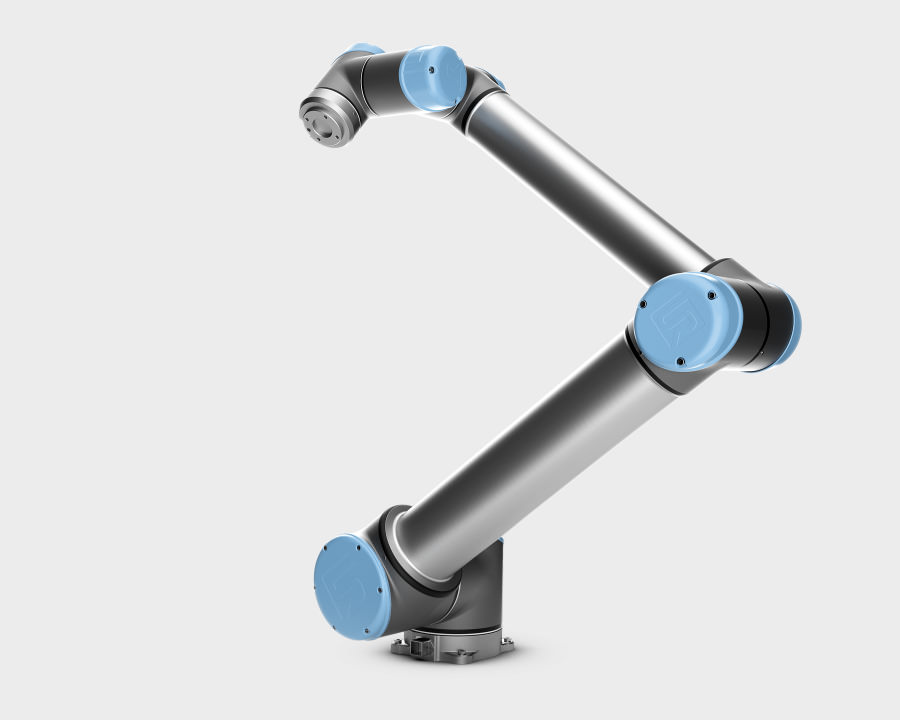
\includegraphics[width=0.7\linewidth]{grafic/ur10_universal_robots}
	\caption{UR10 der Firma Universal Robots, Quelle: \url{https://www.universal-robots.com/3d/images/slider/ur10/small_images/rendersd_00009.jpg}}
	\label{fig:ur10}
\end{figure}


\section{Modellbildung des UR10}

Für die erste Aufgabe soll der Roboter in der Matlab Simulationssoftware Simscape modelliert werden.
Anders als in der Aufgabenstellung angegeben, existiert jedoch nur eine einzelne step-Datei über den gesamten Roboter als Download, welche alle Armteile enthält.
%und nicht aufgeteilt in die einzelnen Armteile als Download.


\subsection{Download und Konvertierung der step-Dateien}
Die step-Datei des UR10 wird auf diversen Webseiten kostenlos zum Download angeboten.
Für das Projekt wurde die Datei der Firma \en{SG-Automatisierungstechnik GmbH}\footnote{\url{https://www.sg-automation.at/}} verwendet.
Die step-Datei lässt sich jedoch nicht direkt in Matlab einlesen, sondern muss mittels des \en{Simscape Multibody Link Plugin} konvertiert werden.
Dabei handelt es sich um ein Zusatzprogramm, welches in bestimmten CAD Anwendungen installiert werden kann und den Export von XML- und Geometriedateien ermöglicht \cite{sm_plugin}.
Als CAD Anwendung für die Konvertierung wurde SolidWorks gewählt. 
Der Dateiexport aus SolidWorks erzeugte eine XML-Datei, eine Geometriedatei \en{UR10\_DataFile.m} sowie acht step-Dateien der verschiedenen Armteile und der Basis.


\subsection{Modellierung in Simscape}

Nun kann die XML-Datei mittels dem Befehl \en{sm\_import()} in Matlab Simscape eingelesen und mit den step-Dateien der Roboterbauteile verknüpft werden.
Nach einer kurzen Sichtung des Modells stellte sich heraus, dass die Transformationen zwischen den Bauteilen zwar korrekt, jedoch die interne Verknüpfung des Blockdiagramms nicht stimmig war.
Beim Einfügen von Aktuatoren bewegte sich ausschließlich das angesteuerte Armteil, während der Rest der kinematischen Kette statisch in der Ausgangsposition verblieb. 

Aus diesem Grund wurde der Import einer URDF-Datei des Roboters versucht, was ebenso über den Befehl \en{sm\_import()} möglich ist.
Die verwendete Datei kann aus dem Github-Repository von \en{Positronics Lab}\footnote{\url{https://github.com/PositronicsLab}}, einer Forschungsorganisation der George Washington Universität, kostenlos heruntergeladen werden.
Hierbei erzeugt Matlab eine eigene XML-Datei, in welcher das Projekt gespeichert ist.
Mit Einfügen der step-Dateien der Armteile erhält man ein funktionierendes Robotermodell des UR10. 
Der originale Output nach Einlesen der URDF-Datei ist in der Abbildung \ref{fig:ur10_origin_modell} zu sehen.
Die Massen und Trägheiten der Armteile wurden aus der zuvor erhaltenen Geometriedatei entnommen.

\begin{figure}[!htbp]
	\centering
	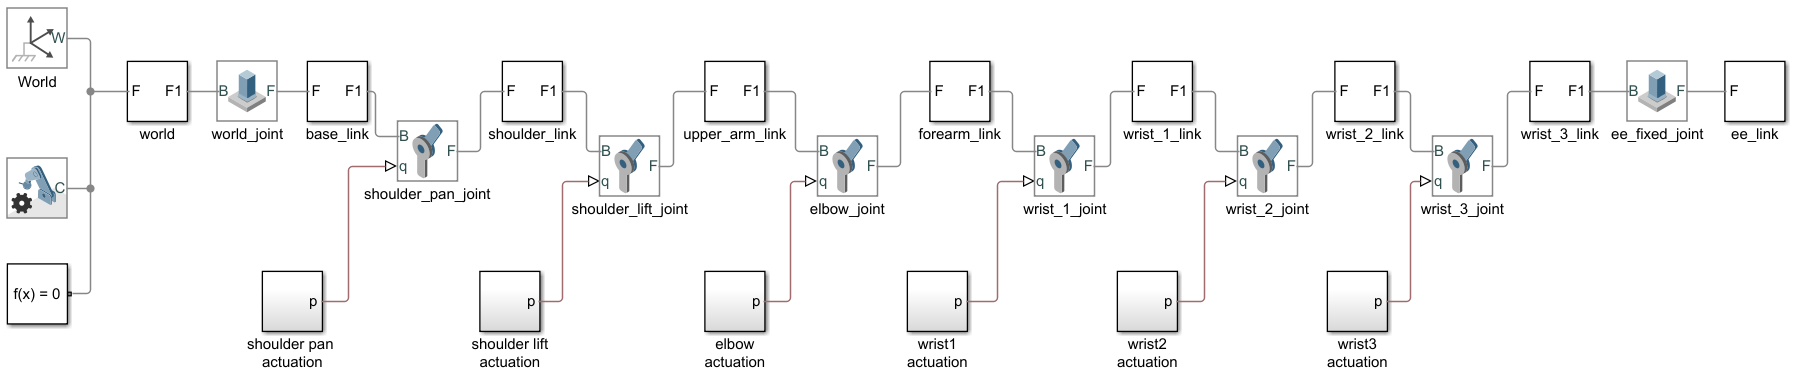
\includegraphics[width=1.0\linewidth]{grafic/origin_UR10_modell}
	\caption{Originales Blockdiagramm des UR10 aus der URDF-Datei}
	\label{fig:ur10_origin_modell}
\end{figure}


\subsection{Integration eines Greifersystems und einer Roboter-Halterung}

Um dem gezeigten Roboter aus dem Beispielvideo möglichst nahe zu kommen, wurde zusätzlich eine Halterung und ein Greifersystem konstruiert.
Die Halterung besteht aus einem quaderförmigen Block, bei dem eine Kante nach oben verschoben ist. % um die schiefe Ebene auf die der Roboter montiert ist zu simulieren.
%Auf der so entstandenen schiefen Ebene ist das Robotermodell wie im Video montiert
Dadurch entsteht eine schiefe Ebene, auf der das Robotermodell wie im Video montiert werden kann.

Das Greifersystem ist aus mehreren Teilen zusammengebaut, einer Werkzeughalterung, zwei Greifern und einem Zylinderstift.
Die Werkzeughalterung ist ein Prisma mit trapezförmiger Grundfläche.
Der Zylinderstift, welcher im Beispielvideo zum Betätigen eines Tasters verwendet wird, ist an einer geraden Fläche an der Haltung befestigt.
Für die beiden seitlich angebrachten Greifer wurde die step-Datei eines möglichst ähnlich aussehenden Greifers von der Website \en{TraceParts}\footnote{\url{https://www.traceparts.com}} verwendet.
Das fertige Robotermodell mit Halterung und Greifersystem ist in Abbildung \ref{fig:ur10_greifer} dargestellt.

\begin{figure}[!htbp]
	\centering
	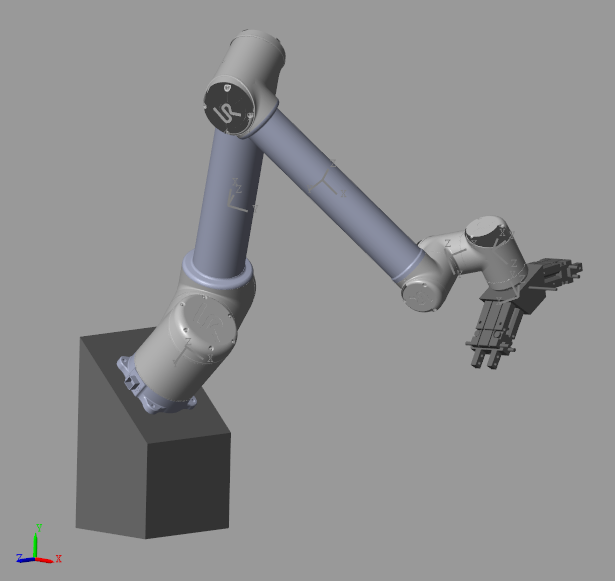
\includegraphics[width=0.5\linewidth]{grafic/UR10_Greifer}
	\caption{UR10 mit Halterung und Greifersystem}
	\label{fig:ur10_greifer}
\end{figure}


\newpage

\subsection{Festlegung der Roboterkoordinatensysteme nach Denavit-Hartenberg-Konvention}

Für die spätere Vergleichsrechnung mit dem Newton-Euler-Verfahren ist es von Vorteil die Koordinatensysteme der Gelenkachsen des Roboters einheitlich zu definieren. %eine einheitliche Festlegung der Koordinatensysteme des Roboters zu definieren.
Hierzu bietet sich die Festlegung nach Denavit-Hartenberg-Konvention an.
Die nachfolgende Abbildung \ref{fig:ur10_dh} zeigt die Koordinatensysteme, wie sie auch im Blockdiagramm definiert sind.

\begin{figure}[!htbp]
	\centering
	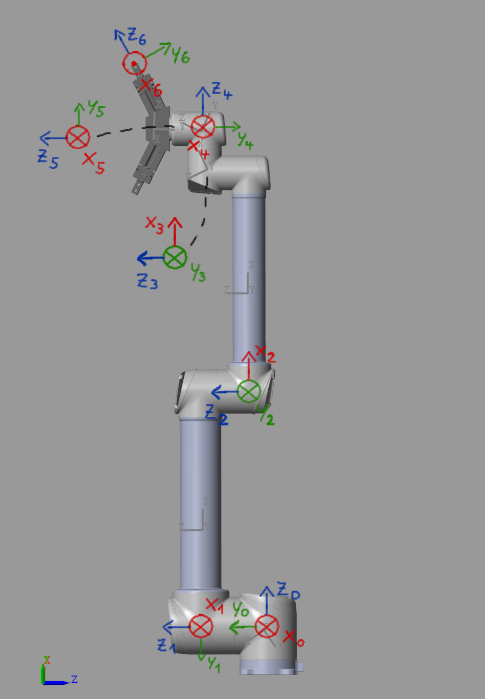
\includegraphics[width=0.5\linewidth]{grafic/UR10_dh}
	\caption{Koordinatensysteme der Gelenke und des TCP nach Denavit-Hartenberg-Konvention}
	\label{fig:ur10_dh}
\end{figure}




\section{Darstellung einer Bewegungssequenz}

Die geforderte PTP Bewegung des Roboters soll die Zeitstempel 1:05 bis 1:08 im Beispielvideo umfassen.
Die daraus resultierende Start- und Endposition ist in den Abbildungen \ref{fig:start_pos} und \ref{fig:end_pos} zusehen.
Die Startposition ist mittig an der Türe, die Endposition an der Steuerung auf der rechten Seite. 
Nach Erreichen der Endposition betätigt der Roboter einen Taster mit seinem am Greifer montierten Zylinderstift und startet dadurch die Werkstückbearbeitung in der Maschine.
Diese Tasterbetätigung ist in der Bewegungssequenz ebenfalls umgesetzt.

\begin{figure}
	\centering
	\begin{subfigure}[b]{0.496\textwidth}
		\centering
		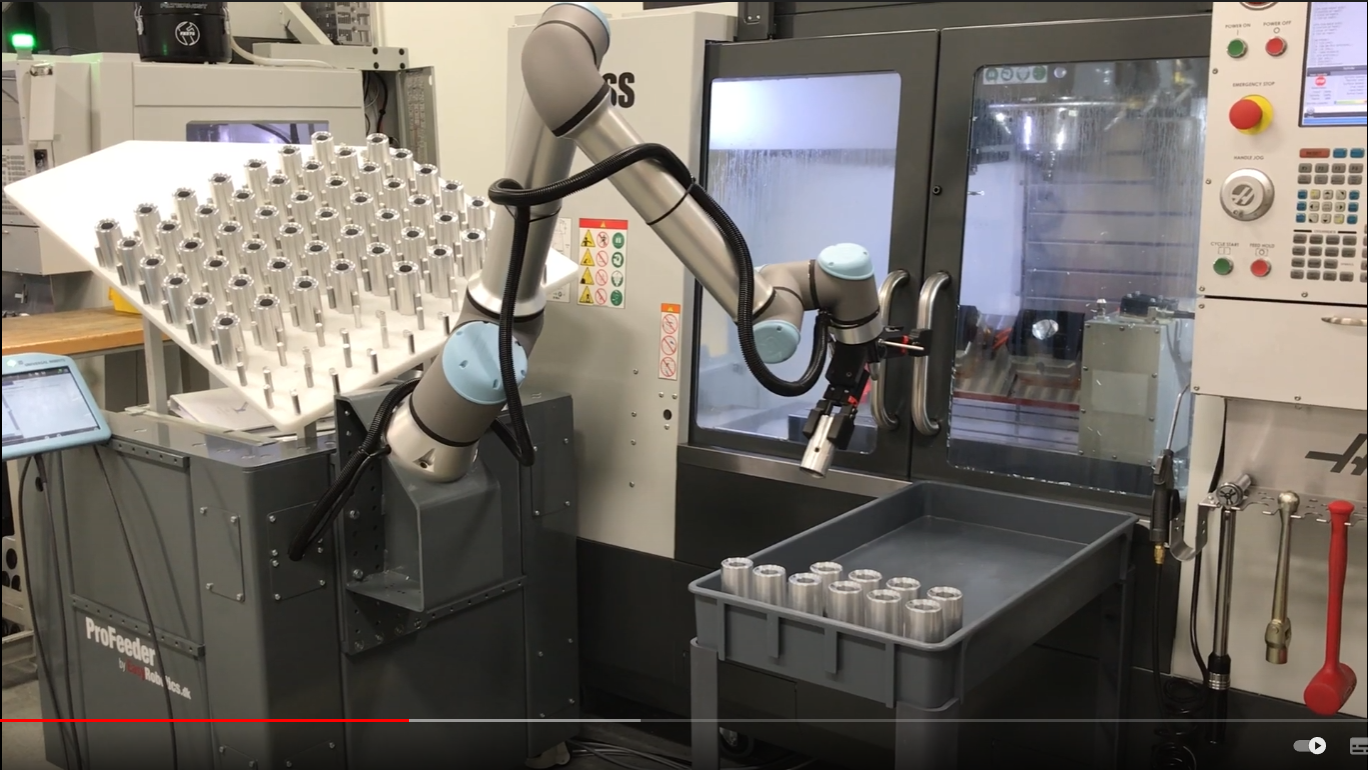
\includegraphics[width=1.0\linewidth]{grafic/ptp_startposition}
		\caption{Startposition}
		\label{fig:start_pos}
	\end{subfigure}
	\begin{subfigure}[b]{0.496\textwidth}
		\centering
		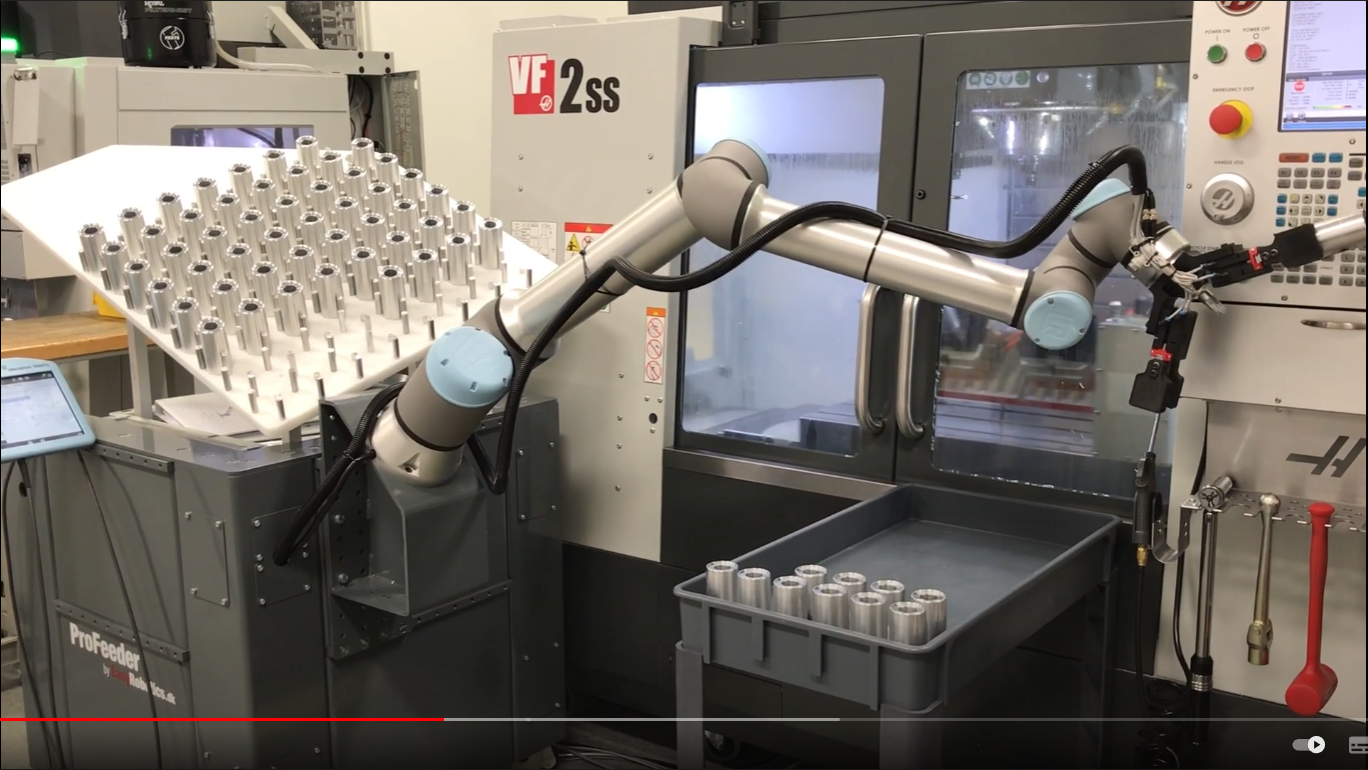
\includegraphics[width=1.0\linewidth]{grafic/ptp_endposition}
		\caption{Endposition}
		\label{fig:end_pos}
	\end{subfigure}
\caption{Start- und Endposition der PTP Bewegung, \\ Quelle: \url{https://www.youtube.com/watch?v=ugxDTtmykE4}}
\label{fig:start_end_pos}
\end{figure}


Die Bewegung ist mittels separater Ansteuerung jeder Gelenkachse realisiert.
Dazu wird ein Block namens \en{Polynominal Trajectory} verwendet, welcher Trajektorien durch gegebene Weg- und Zeitpunkte generiert.
Der verwendete Block ist in Abbildung \ref{fig:ur10_trajectoriengenerator} auf der linken Seite zu sehen.
In unserem Fall handelt es sich bei den Wegpunkten um Winkelstellungen des Gelenks.
Daher ist nach dem Trajektoriengenerator ein \en{Simulink-PS-Converter} eingefügt, der das resultierende einheitenlose Signal des Generators in ein pysikalisches mit der Einheit Rad umwandelt.

\begin{figure}[!htbp]
	\centering
	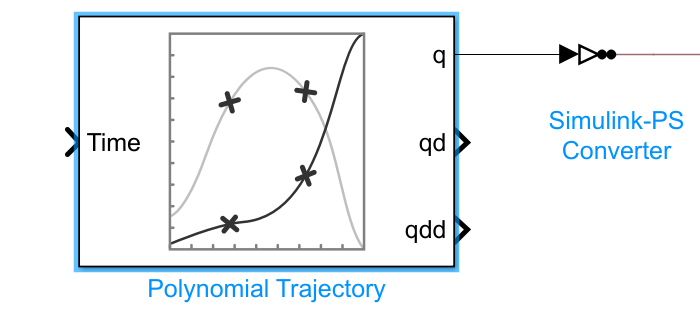
\includegraphics[width=0.55\linewidth]{grafic/Trajectoriengenerator}
	\caption{Blockdiagramm des Aktuators des ersten Gelenks}
	\label{fig:ur10_trajectoriengenerator}
\end{figure}


Für die erste Gelenkachse sind die folgenden Zahlenwerte für die Weg- und Zeitpunkte eingetragen:

\begin{quote}
$Wegpunkte: [0, 0.61, 0.61, 0.52, 0.52, 0.576, 0.576, 0.52, 0.52, 0] $ \\
$Zeitpunkte: [0, 1, 2, 5, 5.5, 6, 6.5, 7, 7.5, 10]$
\end{quote}

Im \en{data\_inspector} von Matlab Simulink kann das erzeugte Signal des Trajektoriengenerators eingesehen werden.
Die Abbildung \ref{fig:data_inspector_rotation_angle} zeigt beispielhaft wieder die erste Gelenkachse.
Zum erleichterten Verständnis sind die verschiedenen Positionen des Roboters und die Betätigung des Tasters im Signal markiert.
%Bei der Home-Position handelt es sich

\begin{figure}[!htbp]
	\centering
	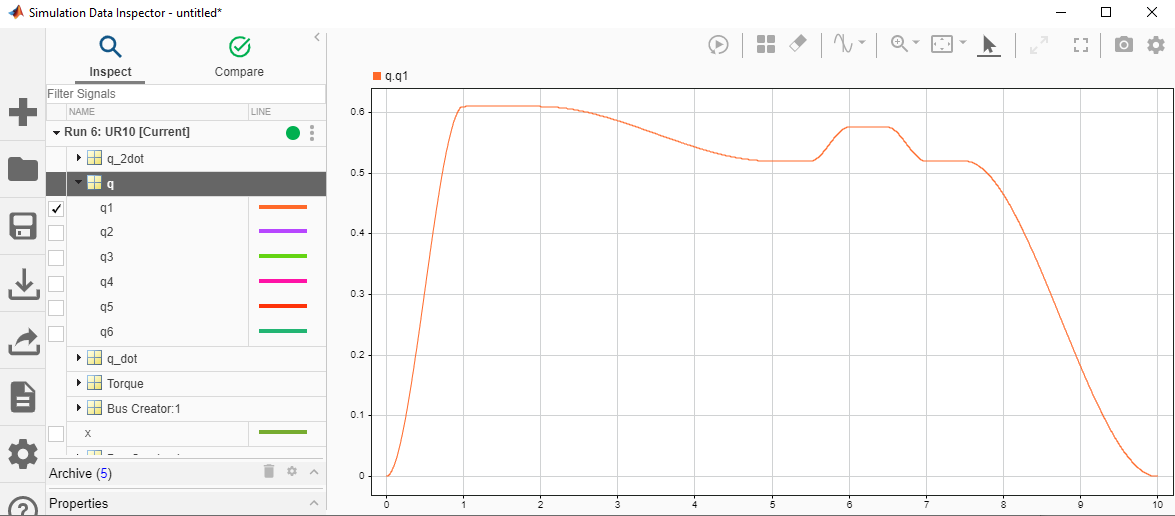
\includegraphics[width=1.0\linewidth]{grafic/data_inspector_Winkel_erstes_Gelenk}
	\caption{Winkelverlauf über Zeit des ersten Gelenks}
	\label{fig:data_inspector_rotation_angle}
\end{figure}


\section{Ausgabe von Drehmomentverläufen}

Damit die Drehmomente der Antriebe in der Simulation ausgegeben werden können, muss die \en{Actuator Torque}-Variable des jeweiligen \en{Revolute Joint} aktiviert werden. 
Die Variable ist im Bereich \en{Sensing} zu finden, wie Abbildung \ref{fig:simscape_revolute_joint_checkbox} zeigt.
Auf Abbildung \ref{fig:simscape_revolute_joint_block} ist der entsprechende Simscape Block mit aktivierter \en{Actuator Torque}-Variable zu sehen.
\noindent
\\[3cm]
\vspace{-3cm}

\begin{figure}
	\centering
	\begin{subfigure}[b]{0.5\textwidth}
		\centering
		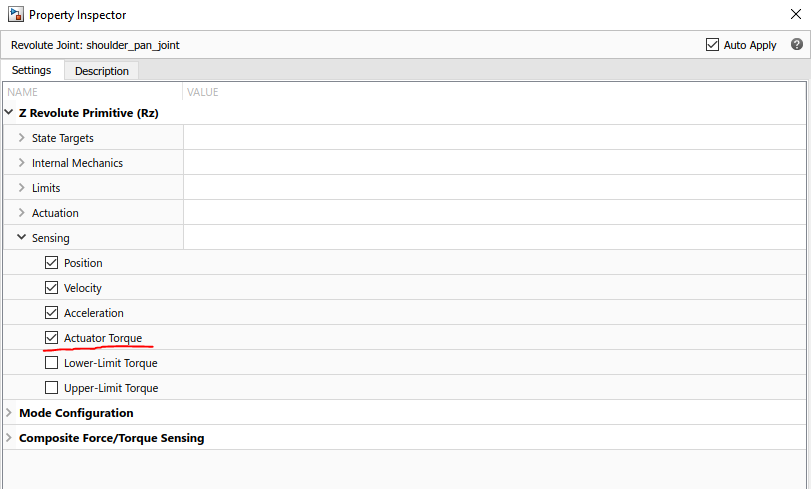
\includegraphics[width=1.0\linewidth]{grafic/actuator_torque}
	\caption{Property Inspector des \en{Revolute Joint}-Blocks mit \en{Actuator Torque}-Checkbox}
	\label{fig:simscape_revolute_joint_checkbox}
	\end{subfigure}
	\begin{subfigure}[b]{0.39\textwidth}
		\centering
		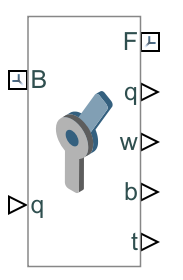
\includegraphics[width=0.3\linewidth]{grafic/revolute_joint}
		\caption{Revolute Joint Simscape Block mit aktivierter \en{Actuator Torque}-Variable}
		\label{fig:simscape_revolute_joint_block}
	\end{subfigure}
	\caption{\en{Property Inspector} des \en{Revolute Joint} und Simscape Block}
\end{figure}

\vspace{2cm}

Danach werden die Ausgaben der Drehmomente aller Gelenke mit dem \en{BusCreator} verbunden, welcher in Abbildung \ref{fig:simulink_logging} auf der linken Seite dargestellt ist.
Die Daten werden dann durch die \en{Log Signals}-Funktion von MATLAB eingeloggt.

\begin{figure}[!htbp]
	\centering
	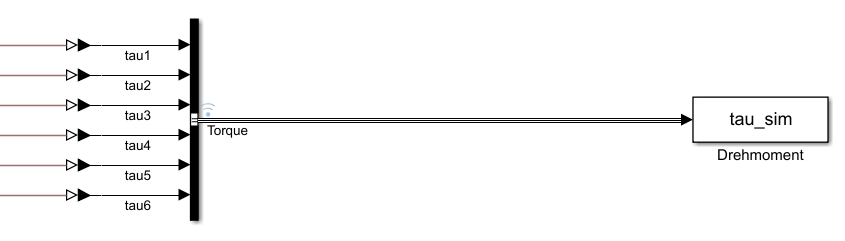
\includegraphics[width=0.8\linewidth]{grafic/torque_busline}
	\caption{Torque Bus Line and Log Sign}
	\label{fig:simulink_logging}
\end{figure}

Die Ergebnisse können im \en{Data Inspector} (Abbildung \ref{fig:drehmomente_simulation}) eingesehen werden.

\begin{figure}[!htbp]
	\centering
	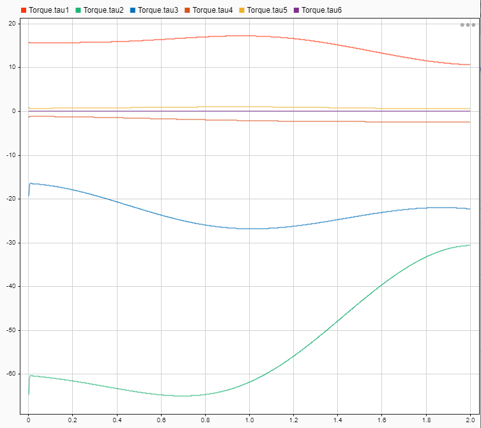
\includegraphics[width=0.5\linewidth]{grafic/Drehmomente}
	\caption{Ausgabe der Drehmomente im \en{Data Inspector}}
	\label{fig:drehmomente_simulation}
\end{figure}


\section{Vergleichsrechnung mit Newton-Euler-Verfahren}

Die Rechnung wird für debugging-Ziele und eine leichtere Simulation (weniger Rechenintensiv) nur nach der Simulation durchgeführt. 
Deswegen sollen die Daten aus der Simulation in den MATLAB-Workspace übertragen werden. 
Für diese Zwecke kann der \en{ToWorkscape} MATLAB-Block verwendet werden, welcher in Abbildung \ref{fig:simulink_to_workspace} dargestellt ist.
Die Daten in dieser Arbeit werden für jeden Zeitpunkt der Simulation gespeichert.

\begin{figure}[!htbp]
	\centering
	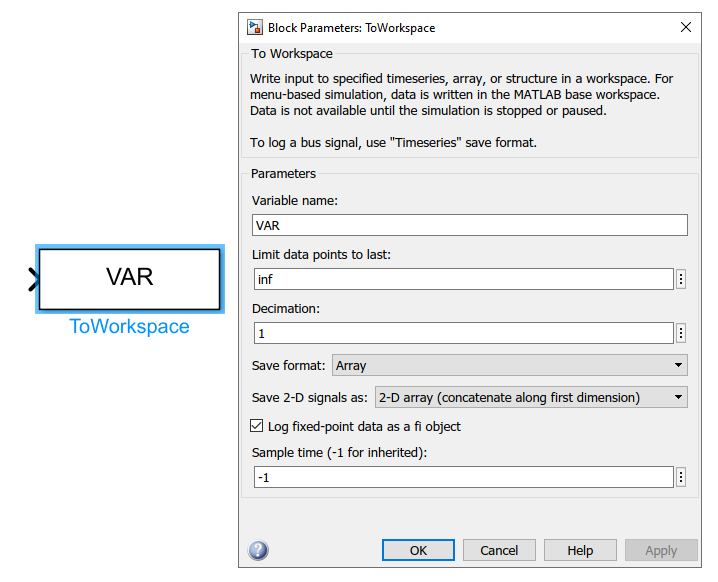
\includegraphics[width=0.59\linewidth]{grafic/to_workspace_block}
	\caption{\en{ToWorkspace}-Block von Matlab}
	\label{fig:simulink_to_workspace}
\end{figure}


\subsection{Abschätzung von Massen und Trägheiten. Ermittlung von Rotationsmatzen, p- und s-Vektoren}

Für die Schätzung der Massen, Trägheiten und s-Vektoren aus der Simulation, steht in Simulink  der \en{Inertia Sensor} zur Verfügung.
Für die Rotationsmatrizen sowie p-Vektoren wird ein \en{Transformation Sensor} verwendet.
Die Sensoren werden in einem Subsystem eingeschlossen. 
Der linke Port des Subsystems entspricht dem Koordinatensystem i, der rechte Port dem Koordinatensystem i+1.
Das Innere des Subsystems ist in der nachfolgenden Abbildung \ref{fig:sensoren_subsystem} zu sehen.

\begin{figure}[!htbp]
	\centering
	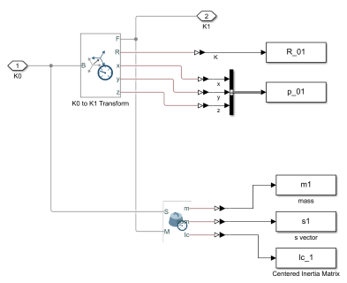
\includegraphics[width=0.54\linewidth]{grafic/sensor_koordinatensystem}
	\caption{Beispiel des Sensorensubsystems}
	\label{fig:sensoren_subsystem}
\end{figure}


\subsection{Berechnung mit Newton-Euler-Verfahren}


\subsubsection{\en{compute\_torques\_with\_newton-euler.m}}

Dieses Skript wird nach der Simulation ausgeführt (StopFnc-Callback in Simulink).
Es führt manche Manipulationen mit den Daten durch, damit sie leichter zu verarbeiten sind.

\begin{lstlisting}[frame=single, basicstyle=\footnotesize, language=Matlab]
if size(q,1) > size(q,2)
q = q';
q_dot = q_dot';
q_2dot = q_2dot';
tau_sim = tau_sim';
end

sim_steps = length(q(1,:));
n_joints = length(q(:,1));

omega = zeros(3, n_joints, sim_steps);
omega_dot = zeros(3, n_joints, sim_steps);
v_dot = zeros(3, n_joints, sim_steps);
vs_dot = zeros(3, n_joints, sim_steps);
tau = zeros(n_joints, sim_steps);

% concatenate data from simulation for easier iteration
R = cat(4, R_01, R_12, R_23, R_34, R_45, R_56);
p = cat(3, p_01', p_12', p_23', p_34', p_45', p_56');
s = cat(3, s1', s2', s3', s4', s5', s6');
Ic = cat(4, Ic_1, Ic_2, Ic_3, Ic_4, Ic_5, Ic_6);
m = cat(1, m1, m2, m3, m4, m5, m6);
m = m';

for i = 1:sim_steps
[omega(:,:,i), omega_dot(:,:,i), v_dot(:,:,i), vs_dot(:,:,i)] = ...
compute_kinematics(q(:,i), q_dot(:,i), q_2dot(:,i), R(:,:,i,:), ...
	R_W0(:,:,i), p(:,i,:), s(:,i,:));
tau(:,i) = compute_forces_and_torques(omega(:,:,i), omega_dot(:,:,i), ...
	vs_dot(:,:,i), m, Ic(:,:,i,:), p(:,i,:), s(:,i,:), R(:,:,i,:));
end

ts = timeseries(tau, tout, 'Name', 'tau');
\end{lstlisting}


\subsubsection{\en{function compute\_kinematics()}}

Die Funktion in Abbildung \ref{fig:sensoren_subsystem_VL} repräsentiert die ersten Schritte des Newton-Euler-Verfahren - \en{kinematische Berechnung}.

\begin{figure}[!htbp]
	\centering
	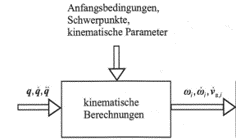
\includegraphics[width=0.42\linewidth]{grafic/compute_kinematics_diagramm}
	\caption{Beispiel des Sensorensubsystems, Quelle: Roboterdynamik, VL 11}
	\label{fig:sensoren_subsystem_VL}
\end{figure}


Die Funktion berechnet die Werte der Geschwindigkeit und Beschleunigungen für K1 mit folgenden Anfangsbedingungen:

\begin{quote}
	$\omega_0 = 0; \hspace{0.5cm} \dot{\omega}_0 = 0; \hspace{0.5cm} \nu = 0; \hspace{0.5cm} \dot{\nu}_0 = -g $
\end{quote}

%\begin{figure}[!htbp]
%	\centering
%	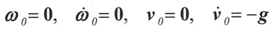
\includegraphics[width=1\linewidth]{grafic/anfangsbedingungen}
%	\caption{Anfangsbedingungen kinematischer Berechnung, Quelle: Roboterdynamik, Vorlesung 11, HHN}
%	\label{fig:anfangsbedingungen}
%\end{figure}


Danach berechnet sie die Werte der Geschwindigkeiten und Beschleunigungen von K2 bis K6 iterativ.

\begin{lstlisting}[frame=single, basicstyle=\footnotesize, language=Matlab]
function [omega, omega_dot, v_dot, vs_dot] = compute_kinematics(q, q_dot, q_2dot, R, R_W0, p, s)
z = [0 0 1]';
n_joints = length(q);

%Anfangsbedingungen
omega = zeros(3, 6);
omega(:,1) = q_dot(1)*z;

omega_dot = zeros(3, 6);
omega_dot(:,1) = q_2dot(1)*z;


% Beschluenigung des KSs.
v_dot(:,1) = inv(R(:,:,1,1)) * (inv(R_W0) * [0 -9.81 0]') + ...
cross(omega_dot(:, 1), p(:,1,1)) + ...
cross(omega(:,1), cross(omega(:,1), p(:,1,1))); 

% Beschleunigung des Schwerpunkts.	
vs_dot(:,1) = v_dot(:,1) + cross(omega_dot(:, 1), s(:, 1, 1)) + ...
cross(omega(:, 1), cross(omega(:,1), s(:, 1, 1))); 

for i = 1:n_joints-1
invR = inv(R(:,:,1,i));

omega(:,i+1) = invR * (omega(:,i) + q_dot(i+1)*z);
omega_dot(:,i+1) = invR * (omega_dot(:,i) + ...
(z * q_2dot(i+1) + cross(omega(:,i), q_dot(i+1) * z)));

v_dot(:, i+1) = invR * v_dot(:,i) + ...
cross(omega_dot(:, i+1), p(:,1,i+1)) + ...
cross(omega(:,i+1), cross(omega(:,i+1), p(:,1,i+1)));
vs_dot(:,i+1) = v_dot(:,i+1) + ...
cross(omega_dot(:, i+1), s(:, 1, i+1)) + ...
cross(omega(:, i+1), cross(omega(:,i+1), s(:, 1, i+1)));
end
end
\end{lstlisting}


Folgende Gleichungen werden in der Funktion verwendet (aus Roboterdynamik, VL 11):

%\begin{quote}
%$\omega_{i+1} = _{i+1}^{i}A$
%\end{quote}
Winkelgeschwindigkeit: 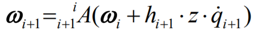
\includegraphics[width=0.4\linewidth]{grafic/omega_gleichung} 

Winkelbeschleunigung: 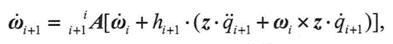
\includegraphics[width=0.6\linewidth]{grafic/omega_dot_gleichung} 

Geschwindigkeit des KSs: 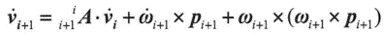
\includegraphics[width=0.64\linewidth]{grafic/v_dot_gleichung}

Geschwindigkeit des Schwerpunkts: 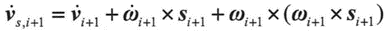
\includegraphics[width=0.63\linewidth]{grafic/vs_dot_gleichung}

%\begin{figure}[!htbp]
%	\centering
%	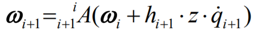
\includegraphics[width=0.5\linewidth]{grafic/omega_gleichung}
%	\caption*{Winkelgeschwindigkeit Gleichung, Quelle: Roboterdynamik, Vorlesung 11, HHN}
%	\label{fig:omega_gleichung}
%\end{figure}
%\begin{figure}[!htbp]
%	\centering
%	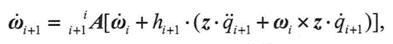
\includegraphics[width=1\linewidth]{grafic/omega_dot_gleichung}
%	\caption{Winkelbeschleunigung Gleichung, Quelle: Roboterdynamik, Vorlesung 11, HHN}
%	\label{fig:omega_dot_gleichung}
%\end{figure}
%\begin{figure}[!htbp]
%	\centering
%	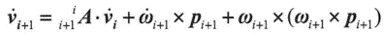
\includegraphics[width=1\linewidth]{grafic/v_dot_gleichung}
%	\caption{Geschwindigkeit des KSs Gleichung, Quelle: Roboterdynamik, Vorlesung 11, HHN}
%	\label{fig:v_dot_gleichung}
%\end{figure}
%\begin{figure}[!htbp]
%	\centering
%	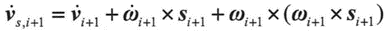
\includegraphics[width=1\linewidth]{grafic/vs_dot_gleichung}
%	\caption{Geschwindigkeit des Schwerpunkts Gleichung, Quelle: Roboterdynamik, Vorlesung 11, HHN}
%	\label{fig:vs_dot_gleichung}
%\end{figure}


\subsubsection{\en{function compute\_forces\_and\_torques()}}

Die Funktion in Abbildung \ref{fig:sensoren_subsystem_foo} repräsentiert den zweiten Schritt des Newton-Euler-Verfahren - \en{Berechnungen der Kräfte und Drehmomente}.

\begin{figure}[!htbp]
	\centering
	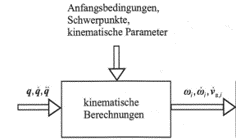
\includegraphics[width=0.43\linewidth]{grafic/compute_kinematics_diagramm}
	\caption{Berechnungen der Kräfte und Drehmomente, Quelle: Roboterdynamik, VL 11}
	\label{fig:sensoren_subsystem_foo}
\end{figure}


\begin{lstlisting}[frame=single, basicstyle=\footnotesize, language=Matlab]
function [tau] = compute_forces_and_torques(omega, omega_dot, vs_dot, m, Ic, p, s, R)
z = [0 0 1]';
n_joints = length(omega(1,:));

% auf n_joints+1 stehen Anfangskraefte- und Drehmomente

f = zeros(3, n_joints+1);
n = zeros(3, n_joints+1);
tau = zeros(1, n_joints);
R(:,:,1,7) = eye(3,3);

for i = n_joints:-1:1
F(:,i) = m(i) * vs_dot(:, i);
f(:,i) = R(:,:,1,i+1) * f(:,i+1) + F(:,i);
N(:,i) = Ic(:,:,1,i) * omega_dot(:,i) + cross(omega(:,i), Ic(:,:,1,i) * omega(:,i));
n(:,i) = n(:,i+1) + cross(p(:,1,i)+s(:,i), F(:,i)) + cross(p(:,i), f(:,i+1)) + N(:,i);
tau(i) = n(:,i)' * inv(R(:,:,1,i)) * z;
end

end
\end{lstlisting}

Folgende Gleichungen werden in der Funktion verwendet (aus Roboterdynamik, VL 11):

%\begin{quote}
%	Kraft an einem Schwerpunkt: $F_{i} = m_i \cdot \dot{\nu}_{s,i}$ 
%\end{quote}

Kraft an einem Schwerpunkt: \; 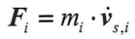
\includegraphics[width=0.15\linewidth]{grafic/Fi_gleichung} 

Gelenkkraft: \; 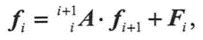
\includegraphics[width=0.28\linewidth]{grafic/klein_fi_gleichung} 

Wirkendendes Drehmoment: 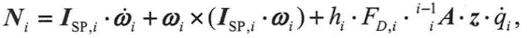
\includegraphics[width=0.62\linewidth]{grafic/gross_n_gleichung} 

Drehmomente im Gelenk: 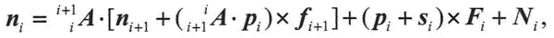
\includegraphics[width=0.68\linewidth]{grafic/klein_n_gleichung} 

Drehmomente im Gelenk: 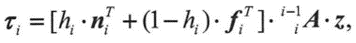
\includegraphics[width=0.5\linewidth]{grafic/tau_gleichung} 

%\begin{figure}[!htbp]
%	\centering
%	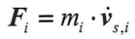
\includegraphics[width=0.15\linewidth]{grafic/Fi_gleichung}
%	\caption*{Kraft an einem Schwerpunkt Gleichung}
%	\label{fig:Fi_gleichung}
%\end{figure}
%\begin{figure}[!htbp]
%	\centering
%	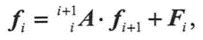
\includegraphics[width=0.28\linewidth]{grafic/klein_fi_gleichung}
%	\caption*{Gelenkkraft Gleichung}
%	\label{fig:klein_fi_gleichung}
%\end{figure}
%\begin{figure}[!htbp]
%	\centering
%	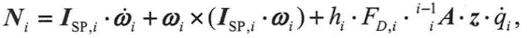
\includegraphics[width=0.55\linewidth]{grafic/gross_n_gleichung}
%	\caption*{Wirkenden Drehmonent Gleichung}
%	\label{fig:gross_n_gleichung}
%\\\end{figure}
%\begin{figure}[!htbp]
%	\centering
%	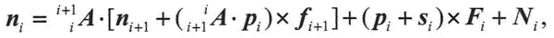
\includegraphics[width=0.6\linewidth]{grafic/klein_n_gleichung}
%	\caption*{Drehmomente in dem Gelenk Gleichung}
%	\label{fig:klein_n_gleichung}
%\end{figure}
%\begin{figure}[!htbp]
%	\centering
%	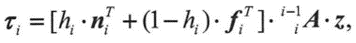
\includegraphics[width=1\linewidth]{grafic/tau_gleichung}
%	\caption{Drehmomente in dem Gelenk Gleichung, Quelle: Roboterdynamik, Vorlesung 11, HHN}
%	\label{fig:tau_gleichung}
%\end{figure}








%\clearpage
%\listoffigures

%\clearpage
%\listoftables


%%%%%%%%%%%%%%%%%%%%%%%%%%%%%%%%%%%%%%%%%%%%%%%%%%%%%
% L I S T   O F   A C R O N Y M S
%%%%%%%%%%%%%%%%%%%%%%%%%%%%%%%%%%%%%%%%%%%%%%%%%%%%%

% @acuda
% Append Acronym-List in Document with \appendix
% for old behavior use \Oldappendix
% acronym should be the name of the appendix file (linux sort hack)
% linux hack: sort unsort.tex -o sorted.tex (should called via sh-script)
% appendix-file entry: \acro{VERWEIS}[ABKÜRZUNG]{AUSGESCHRIEBEN}
% use acronym:
%   \ac{lable}      full name only at first usage in text
%   \acs{lable}     short name only
%   \acf{lable}     short and full name only
%   \acl{lable}     full name only
%\clearpage
%\phantomsection \addcontentsline{toc}{section}{Acronyms}
%\begingroup
%	\renewcommand\refname{Acronyms} \section*{Acronyms}
%	\sectionmark{Acronyms}
%	% Format der Abkürzungsdefinition: \acro{}[]{}
%	% {Verweis}[Abkürzung]{ausgeschriebene Abkürzung}
%	\begin{acronym}[Library-BindingW] %NMWC YTM
%		\leftskip1.5em
%		\setlength{\itemsep}{-\parsep}
%			\acro{dm}[DM]{dm-drogerie markt GmbH + Co. KG}
%			\acro{eu}[EU]{European Union}
%			\acro{gbs}[GBS]{\en{Green Bag Solutions GmbH}}
%			\acro{kik}[KiK]{KiK Textilien und Non-Food GmbH}
%			\acro{smart}[SMART]{Specific Measurable Accepted Realistic and Time}
%			\acro{wbs}[WBS]{\en{Work Breakdown Structure}}
%			\acrodefplural{wbs}[WBSs]{\en{Work Breakdown Structures}}
%			\acro{lip}[LiP]{\en{Leading in Projects}}
%	\end{acronym}
%\endgroup


\clearpage

\singlespacing

\renewcommand{\refname}{Literaturverzeichnis}
\bibliography{bibliography}
\bibliographystyle{alphadin}


%}
%
%
%\clearpage
%\input{appendix/_appendix}


\end{document}
